\chapter{Experimentos e Resultados}
\label{chap:resultados}
% ----------------------------------------------------------
Este capítulo vem apresentar os experimentos realizados como forma de
verificação do Processo de Avaliação de Capacidade por Inferência de 
Desempenho proposto no Capítulo~\ref{chap:processo}. Inicialmente é
apresentada a metodologia utilizada para construção dos experimentos, 
com a descrição da Aplicação sob Teste escolhida, como foi implantada e 
como foram realizadas as execuções para coleta de dados de desempenho. Depois
são apresentados os resultados obtidos por cada uma das 9 Heurísticas ao
fazer a Avaliação de Capacidade da Aplicação. Esses resultados são usados 
para uma comparação qualitativa das Heusrísticas entre si e para atestar
a eficiência do Processo de Avaliação de Capacidade proposto e sua técnica 
de Inferência de Desempenho tanto quanto à economia de tempo e custo como  
quanto à precisão de acerto de seuas predições.

\section{Metodologia}
\label{sec:resultados_metodologia}
A fim de validar a eficiência da Inferência de Desempenho no apoio
ao Planejamento de Capacidade, foram realizadas seções de avaliação de
capacidade de uma aplicação implantada em um provedor de nuvem de
infraestrutura como serviço.

A aplicação escolhida foi o WordPress \cite{wordpress}, um motor de construção 
e administração de \emph{blogs}. Sua escolha foi motivada por ser uma aplicação
bem conhecida, de utilização via web, ideal para implantação em ambiente de
nuvem, e com componentes arquiteturais escaláveis. Além disso, o fluxo de 
utilização típico apresenta características bem diversificadas quanto ao uso
de recursos de CPU e memória, rede, sistema de arquivos e banco de dados.

\begin{figure}[htb]
  \caption{\label{fig:implantacao}Implantação do WordPress na AWS EC2 para Avaliação de Capacidade}
  \begin{center}
    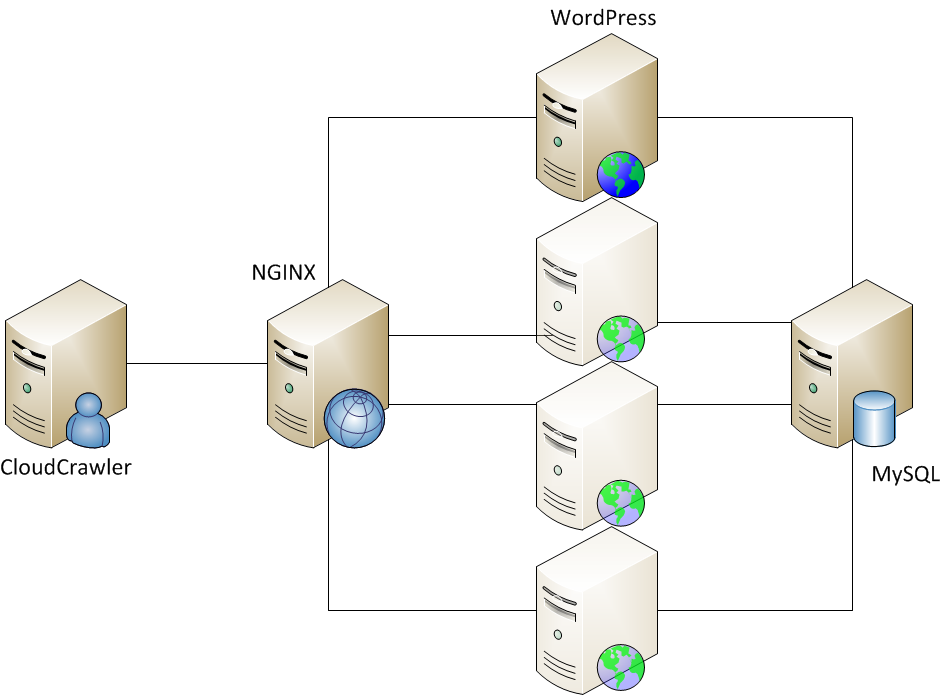
\includegraphics[scale=0.5]{img/ImplantacaoWordPress}
  \end{center}
\end{figure}

O Provedor escolhido foi a Amazon, com seu serviço de infraestrutura AWS EC2
\cite{ec2}, onde o WordPress foi implantado em duas camadas: uma para o banco de 
dados MySQL, e outra para a aplicação, executada pelo servidor Apache HTTPD. Como
balanceador de carga, foi utilizada uma máquina executando o servidor web Nginx. A
Figura~\ref{fig:implantacao} mostra um panorama geral dessa implantação. 

%Na imagem,
%podem ser vistos que na camada do WordPress algumas máquinas aparecem esmaecidas.
%Isso foi feito para representar que os testes variam


% ----------------------------------------------------------
